%%%%%%%%%%%%%%%%%%%%%%%%%%%%%%%%%%%%%%%%%
% Twenty Seconds Resume/CV
% LaTeX Template
% Version 1.0 (14/7/16)
%
% This template has been downloaded from:
% http://www.LaTeXTemplates.com
%
% Original author:
% Carmine Spagnuolo (cspagnuolo@unisa.it) with major modifications by 
% Vel (vel@LaTeXTemplates.com)
%
% License:
% The MIT License (see included LICENSE file)
%
%%%%%%%%%%%%%%%%%%%%%%%%%%%%%%%%%%%%%%%%%

%----------------------------------------------------------------------------------------
%	PACKAGES AND OTHER DOCUMENT CONFIGURATIONS
%----------------------------------------------------------------------------------------

\documentclass[letterpaper]{twentysecondcv} % a4paper for A4

%bibliogrphy
\usepackage[utf8]{inputenc}
\usepackage{doi}
\usepackage[style=numeric,sorting=ydnt,maxbibnames=9,backend=biber,doi=false,
isbn=false,date=year,block=space]{biblatex}
\setlength\bibitemsep{0.2cm}
\usepackage{setspace}
%\usepackage[style=bwl-FU,maxbibnames=100,maxcitenames=1,backend=biber,doi=false,isbn=false,url=false,date=year,block=space]{biblatex}
\addbibresource{references.bib}

%----------------------------------------------------------------------------------------
%	 PERSONAL INFORMATION
%----------------------------------------------------------------------------------------

% Define custom commands for CV info
\newcommand{\cvmail}[1]{\renewcommand{\cvmail}{#1}}
\newcommand{\cvnumberphone}[1]{\renewcommand{\cvnumberphone}{#1}}
\newcommand{\cvsiteRG}[1]{\renewcommand{\cvsiteRG}{#1}}
\newcommand{\cvsiteLN}[1]{\renewcommand{\cvsiteLN}{#1}}



\cvsiteLN{javier-gracia-tabuenca-7b411029}
\cvnumberphone{+358 469 086 981} % Phone number
\cvsiteRG{Javier\_Gracia2} % Personal website
\cvmail{javier.gracia.tabuenca@gmail.com} % Email address


\begin{document}
%----------------------------------------------------------------------------------------
%	 TITLE
%----------------------------------------------------------------------------------------
\makeprofileTitle{Javier Gracia-Tabuenca}

%----------------------------------------------------------------------------------------
%	 Left page 1
%----------------------------------------------------------------------------------------
\begin{LeftPage1} % Print the sidebar
%
\profilepic{img/pic.jpg}

\jobtitle{~\\Biomedical R\&D \\ HW and signal-processing}

\begin{spacing}{0.4}

	\cvlink{\small\cvsiteLN}
	{https://www.linkedin.com/in/\cvsiteLN}
	{img/ln.png}
		
	\cvlink{\normalsize\cvsiteRG}{https://www.researchgate.net/profile/\cvsiteRG}{img/researchgate_grey_2.png}

	\cvlink{\normalsize\cvnumberphone}{\cvnumberphone}{img/tel.png}

	\cvlink{\small \cvmail}{mailto:\cvmail}{img/email.png}

\end{spacing}



%KNOWLEDGE
\profilesection{Knowledge}{3cm}

\skills

%PROGRAMING
\profilesection{Programming}{2.2cm} 
        
\lanprog{Matlab}{+6y}{Signal processing, chaos analysis} 
\lanprog{R}{+2y}{Statistical analysis}    
\lanprog{C}{+2y}{MSP430, ESP8266, Arduino}
\lanprog{LabView}{+2y}{USB-6259, PID, +Matlab}
\lanprog{Altium}{+2y}{PCB, also Eagle}
\lanprog{Comsol}{+1y}{3D thorax, AC/DC, +Matlab}
        %\lanprog{git,}{}{}

\end{LeftPage1}

%----------------------------------------------------------------------------------------
%	 Right page 1
%----------------------------------------------------------------------------------------
\begin{RigthPage1}
%----------------------------------------------------------------------------------------
%	 Profile
\section{Profile}  
Spanish electrical engineer     Hands-on experience on a wide spectrum of the R\&D cycle of medical devices. Ranging from hardware design to patient testing, including advance signal processing methods and statistical analysis. 
\\
%----------------------------------------------------------------------------------------
%	 WORK
\section{Work Experience}        
\begin{twenty}
	\twentyitemlist
    	{2018}
        {Scientific Advisor}
        {\href{https://www.ventica.net/}{\textbf{Ventica®}}} 
        {
          \item Consultancy algorithm development.
        }
        
	\twentyitemlist
    	{2013 - 2019}
        {Researcher PhD.}
        {\href{https://www.tut.fi/}{\textbf{Tampere University of Technology}}}
        {
          \item Signal-processing \& HW design.
          \item See projects section below.
        }
        
	\twentyitemlist
    	{2013 - 2019}
        {Lecturer}
        {\href{https://www.tut.fi/}{\textbf{Tampere University of Technology}}}
        {
        \item Lecture and assist students on various medical HW/SW projects.  
        \item Main responsible of 
\href{https://www.youtube.com/watch?time_continue=1&v=E3D8rAG6S4Q}{“Basics of Medical Electronics” }.
        %\\   \href{https://eacea.ec.europa.eu/sites/2007-2013/tempus-programme_en}{TEMPUS} program: U. of Montenegro, U. of Belgrade. 
        }

	\twentyitemlist
    	{2012 - 2013}
        {Researcher}
        {\href{https://www.tut.fi/}{\textbf{Tampere University of Technology}}}
        {
        \item Testing wearable's firmware, now knows as \href{https://www.ventica.net/}{Ventica®}.   }

	\twentyitemlist
    	{2011 - 2012}
        {Researcher}
        {\href{https://http://www.fcirce.es//}{\textbf{Fundaci\'on CIRCE}}}
        {
        \item Write optimization algorithms.
        }
\end{twenty}

%----------------------------------------------------------------------------------------
%	 Proyects 
\section{Projects}
\begin{twenty} % Environment for a list with descriptions
	\twentyitemlist
    	{2017 - 2019}
        {Asthma assessed from nocturnal tidal breathing in children~\cite{children,infants}}
        {\\Collaboration: Helsinki university hospital, Tampere university hospital }
        {
        \item Respiration feature extraction.
        \item Sleep phase detection.
        \item Statistical analysis.
        \item Manuscript writing.
        %Algorithms defining sleep phase, algorithms measuring breath-to-breath parameters, signal processing, statistical analysis, hardware testing, manuscript writing.
        %I designed algorithms defining sleep phases and measuring breath parameters. I carry statistical analysis to find the best parameters and sleep time to monitor asthma. I run the code in a AWS-like sys.
        }
        

	\twentyitemlist
    	{2016 - 2017}
        {Nonlinear local projection filter for impedance pneumography~\cite{nlpf}}
        {\\Collaboration: Tampere university hospital }
        {
        \item Write algorithm borrowed from chaos analysis
        \item Test method on respiratory flow.
		%This noise reduction method, borrowed from chaos analysis, has a great potential for biosignals. I demonstrated so for respiratory flow. 
		}
       
  
  \twentyitemlist
    	{2013 - 2016}
        {Combined impulse oscillometry-impedance pneumography~\cite{iosj,multi}}
        {}
        {
        %I designed, building, and calibrated the electronics, mechanics, and signal processing. I designed and carried a test in healthy volunteers.
        \item Design hardware. 
        \item Test hardware. 
        \item Implement signal processing
        \item Conduct test in healthy volunteers
        }       
\end{twenty} 
%----------------------------------------------------------------------------------------
%	 Foot
\begin{flushright}
\textbf{\textit{For publications [$\cdot$] consult the next page}}
\\
\textbf{\textit{For interactive links consult the PDF version}}
\end{flushright}
% \clearpage
\end{RigthPage1}


\newpage


%----------------------------------------------------------------------------------------
%	 Left page 1
%----------------------------------------------------------------------------------------
\begin{LeftPage2} % Print the sidebar
%Languages         
\profilesection{Languages}{3cm} 
              

\includegraphics[width=1.2cm]{img/esp.png}~

\includegraphics[width=1.4cm]{img/eng.png}~

\includegraphics[width=1.2cm]{img/cat.png}~

\includegraphics[width=1.2cm]{img/fin.png} 
  
%----------Interest-------------------------------------- 
\vspace{1cm}     
\profilesection{Interests}{3.6cm}   
\begin{center}   
   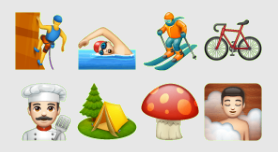
\includegraphics[width=4.5cm]{img/test.png}
\end{center}

\end{LeftPage2}



%----------------------------------------------------------------------------------------
%	 Right page 1
%----------------------------------------------------------------------------------------
\begin{RigthPage2}
%----------------------------------- EDUCATION ------------------------------------------
\section{Education}


\begin{twenty} % Environment for a list with descriptions
	\twentyitemlist
    	{2013 - 2019}
        {PhD. Biomedical Engineering}
        {\href{https://www.tut.fi/}{\textbf{Tampere University of Technology}}}
        {
        \item Specialization: Novel hardware and signal processing for paediatric lung function testing based on impedance pneumography.}
	\twentyitemlist
    	{2005 - 2009}
        {MSc. Electronics Engineering}
        {\href{https://www.upc.cat}{\textbf{Universitat Politecnica de Catalunya}}}
        {
        \item Master's thesis at: Tampere University of Technology.
        \item Awards: 3rd best grade of the 15th graduation year.
        }
     \twentyitemlist
    	{2000 - 2005}
        {BEng. Computer Sciences }
        {\href{http://www.unizar.es/}{\textbf{Universidad de Zaragoza } }}
        {
        \item Awards: Best bachelor's thesis 2004/2005, Awarded by \href{http://www.aitia.org/}{AITIA}.}
	%\twentyitem{<dates>}{<title>}{<organization>}{<location>}{<description>}
\end{twenty}

%-------------------------------- Conferences-----------------------------------------

\section{Conferences }

\begin{twenty} % Environment for a list with descriptions

	\twentyitem
    	{Jun 2018}
        {IUPESM2018, World congress biomedical engineering}
        {Prague, Czech Republic}
        {\href{https://www.slideshare.net/slideshow/embed_code/key/z0l5pXuzNVj5EG}{Oral presentation}}
        

	\twentyitem
    	{Jun 2017}
        {EMBEC17, European medical engineering conference~\cite{nlpf}}
        {Tampere, Finland}
        {\href{https://www.slideshare.net/slideshow/embed_code/key/34qLaFcP2gR6ji}{Oral presentation}}
      

	\twentyitem
    	{Feb 2015}
        {ICBEM, International conference on bioelectromagnetism~\cite{iosc}}
        {Tallin, Estonia}
         {\href{https://www.slideshare.net/slideshow/embed_code/key/bRO5NrltJZFizD}{Oral presentation} }       
               

	\twentyitem
    	{Sep 2013}
        {ERS congress 2013, European respiratory society~\cite{iosers}}
        {Barcelona (Spain)}
        {\href{http://www.ers-education.org/Media/Media.aspx?idMedia=228641}{Poster presentation}  }      
        
        
\end{twenty}    
\end{RigthPage2}
      
        

%----------------------------------------------------------------------------------------
%	 bibliography 
%----------------------------------------------------------------------------------------

\begin{downPubli}

\section{Publications}

\nocite{*}

\printbibliography[heading=none,title={}]

\begin{flushright}
\textit{* unpublished}
\end{flushright}
\end{downPubli}


\end{document} 
